MPEG-7 es un estándar para la descripción de contenido multimedia, que define un conjunto de atributos simples y de bajo nivel con el propósito de caracterizar cualquier tipo de sonido.
Este conjunto está constituido por 17 características asociadas a toda señal de sonido~\cite{Kim05,Manjunath02}.
A continuación presentamos una descripción de estas, agrupándolas de acuerdo al modo en que describen la señal.

\subsection{Descriptores básicos}\label{subsec:descriptoresBásicos}

Las dos características de esta categoría describen las propiedades de la señal en el dominio del tiempo de forma simple;
el costo computacional de calcularlas es bajo.

\subsubsection{Audio Waveform}

Para computar esta característica se divide la señal en tramas no superpuestas ($M = N$), y se computan, por cada trama, los 2 valores siguientes:

\begin{itemize}
    \item Menor valor de amplitud de la señal presente en la trama.
    \item Mayor valor de amplitud de la señal presente en la trama.
\end{itemize}

El \textit{audio waveform} (AWF) de la señal consistirá en un vector con los pares calculados, correspondientes a cada una de dichas tramas.

La extracción de esta característica puede ser vista como un modo de <<compresión>> de la señal.
Si se toma $N=1$ se obtendrá la propia señal, mientras que a medida que se seleccionen valores de $N$ más altos, el número de valores resultantes será cada vez menor, obteniéndose una representación reducida de la señal original.
El AWF puede representarse gráficamente como un conjunto de segmentos con extremos en los valores de la tupla correspondiente y desplazados en el tiempo relativo a su posición en la señal (figura~\ref{img:awf+ap}).

\subsubsection{Audio Power}

El \textit{audio power} (AP) describe el comportamiento de la potencia de la señal en cada instante de tiempo.
Al igual que para la AWF, su cálculo requiere dividir la señal en tramas no superpuestas;
y se computa, para la trama $x[n]$ mediante la siguiente expresión:

\begin{equation}
    \label{eq:AP}
    AP = \frac{1}{N}\sum_{n=0}^{N-1}{|x[n]|^2}
\end{equation}

La representación gráfica del AP posibilita el análisis directo de la evolución de la amplitud de la señal en el transcurso del tiempo, lo que puede observarse en la figura~\ref{img:awf+ap}.

\begin{figure}[!h]
    \centering
    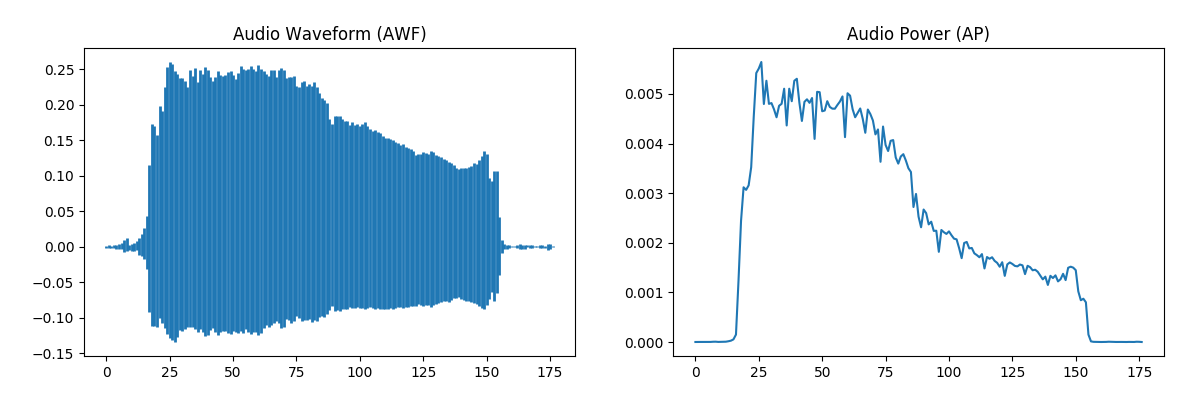
\includegraphics[width=\textwidth]{awf+ap.png}
    \caption{Características básicas de una señal de audio según MPEG-7.}
    \label{img:awf+ap}
\end{figure}

